\begin{problem}[16]
什么条件下可以不考虑表面张力对水波波速的影响, 从物理上作简单分析.
\end{problem}
% --------------------------------------------------------------------
\begin{solution}
水波在水面传播的过程主要由于惯性和恢复力共同作用引起的. 恢复力主要是重力和水的表面张力(波长较长时忽略), \textbf{定性分析}:

\vspace{5pt}

\noindent
\begin{minipage}[c]{0.7\linewidth}
\begin{itemize} 
\item 当波长$\lambda$较长, 使水面恢复平面形状的恢复力主要是重力, 相比于重力和惯性, 表面张力微不足道, 可以不考虑. 
\item 当波长$\lambda$较短, 水的表面张力也是一种使水面恢复平面形状的有效恢复力, 此时必需考虑表面张力.
\end{itemize}
\end{minipage}
\begin{minipage}[c]{0.3\linewidth}
\begin{center}
\usetikzlibrary{calc,intersections,through,backgrounds}
\usetikzlibrary{decorations.pathreplacing,decorations.pathmorphing,arrows}
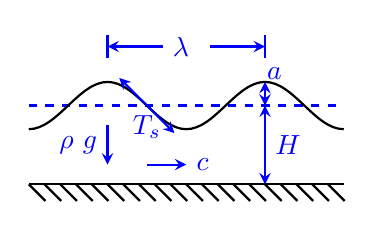
\begin{tikzpicture}[ media/.style={font={\footnotesize\sffamily}},
    interface/.style={
        postaction={draw,decorate,decoration={border,angle=-45,
                    amplitude=0.3cm,segment length=2mm}}}]
\draw[thick,interface] (-2,0)--(2,0);
\draw[thick,dashed,blue](-2,1)--(2,1);
%\draw[thick] (-2,0.75) arc (-90:-15:0.5 and 0.25); %arc(180:0:0.5 and 0.25);
\draw[thick] (-2,0.7) cos (-1.5,1) sin(-1,1.3) cos(-0.5,1) sin(0,0.7) cos(0.5,1) sin(1,1.3) cos(1.5,1) sin(2,0.7);
\draw [thick,blue] (-1,1.6) -- (-1,1.9) (1,1.6) -- (1,1.9);
\draw [thick,blue,<-,>=stealth] (-1,1.75) -- (-0.3,1.75) node[right]{$\lambda$};
\draw [thick,blue,<-,>=stealth] (1,1.75) -- (0.3,1.75);
\draw [thick,blue,<->,>=stealth] (-0.15,0.65)--(-0.85,1.35) node[below,midway]{$T_s$};
\draw [thick,blue,<->,>=stealth] (1,0)--(1,1) node[right,midway]{$H$};
\draw [thick,blue,<->,>=stealth] (1,1)--(1,1.3) node[above right=-3pt]{$a$};
\draw [thick,blue,->,>=stealth] (-0.5,0.25)--(0,0.25) node[right] {$c$};
\draw [thick,blue,->,>=stealth] (-1,0.75)--(-1,0.25) node[midway,left] {$\rho$ $g$};
\end{tikzpicture}
\end{center}
\end{minipage}\vspace{10pt}

\noindent
下面分别从量纲分析角度和水波理论角度进行讨论:
\begin{itemize}
\item \textbf{量纲分析:}
水波波速$c$与水的密度$\rho$, 表面张力$T_s$, 重力加速度$g$, 水波波长$\lambda$, 波幅$a$, 水深$H$有关:
\[
c = f(\rho,g,\lambda,a,H,T_s)
\]
上式中各物理量的量纲分别为: $[c]=LT^{-1}$, $\rho=ML^{-3}$, $[g]=LT^{-2}$, $[\lambda]=[a]=[H]=L$, $[T_s]=MT^{-2}$. 选取$\rho$, $g$, $H$作基本量, 并作为本问题的单位系统, 用以度量问题中的各量, 于是, 上式转化为
\[
\frac{c}{\sqrt{gH}} = f\bigg(1,1,\frac{\lambda}{H}, \frac{a}{H}, 1, \frac{T_s}{\rho g H^2}\bigg) = f\bigg(\frac{\lambda}{H},\frac{a}{H},\frac{T_s}{\rho g \lambda^2}\cdot\Big(\frac{\lambda}{H}\Big)^2\bigg) = f\bigg(\frac{\lambda}{H}, \frac{a}{H}, \frac{T_s}{\rho g \lambda^2}\bigg)
\]
观察上式不难发现: 当$\lambda\gg \sqrt{T_s/(\rho g)}$, 即波长$\lambda$较大时, 表面张力对水波波速的影响可以不考虑.

\item \textbf{水波理论:}
水波理论给出$f$的形式是
\[
\frac{c}{\sqrt{gH}} = \bigg[1+\frac{(2\pi)^2T_s}{\rho g \lambda^2}\bigg]^{1/2}\bigg[\frac{2\pi H/\lambda}{2\pi H/\lambda}\bigg]^{1/2}
\]
从上式中的右端第一个因子也可以看出, 当$\frac{(2\pi)^2T_s}{\rho g \lambda^2}\ll 1$即$2\pi\sqrt{T_s/(\rho g)}\ll \lambda$时, 表面张力对水波波速的影响可以不考虑.
\end{itemize}
综上所述, 无论是从定性分析, 还是量纲分析及水波理论, 都可以得出: \textbf{当水波波长较长时, 可以不考虑表面张力对水波波速的影响}.
\end{solution}
